\section{Metodologia}
\subsection*{Metodologia}

\begin{frame}{{\sffamily Metodologia de Pesquisa}}
  \begin{block}{}
    Adaptação da classificação por Prodanov e Freitas:
    \begin{itemize}
      \item Abordagem qualitativa e quantitativa %
      \item Natureza aplicada: % Pesquisa aplicada, aplicar conhecimentos/resultados gerados em problemas específicos
            \SubItem{Geração de um produto}
      \item Quanto aos Objetivos: % Exploratória, utilizar os dois metodos para coletar informações para construir uma ferramenta melhor.
            \SubItem{Pesquisa exploratória}
      \item Quanto aos Procedimentos: %Documental literatura cinza, Estudo de caso coletar informações diretamente do usuário, Survey, teve teste piloto tbm.
            \SubItem{Documental - literatura cinza}
            \SubItem{Levantamento}
            \SubItem{Estudo de caso}

    \end{itemize}
  \end{block}
\end{frame}

\begin{frame}{{\sffamily Desenho de Pesquisa}}
  \begin{figure}
    \centering
    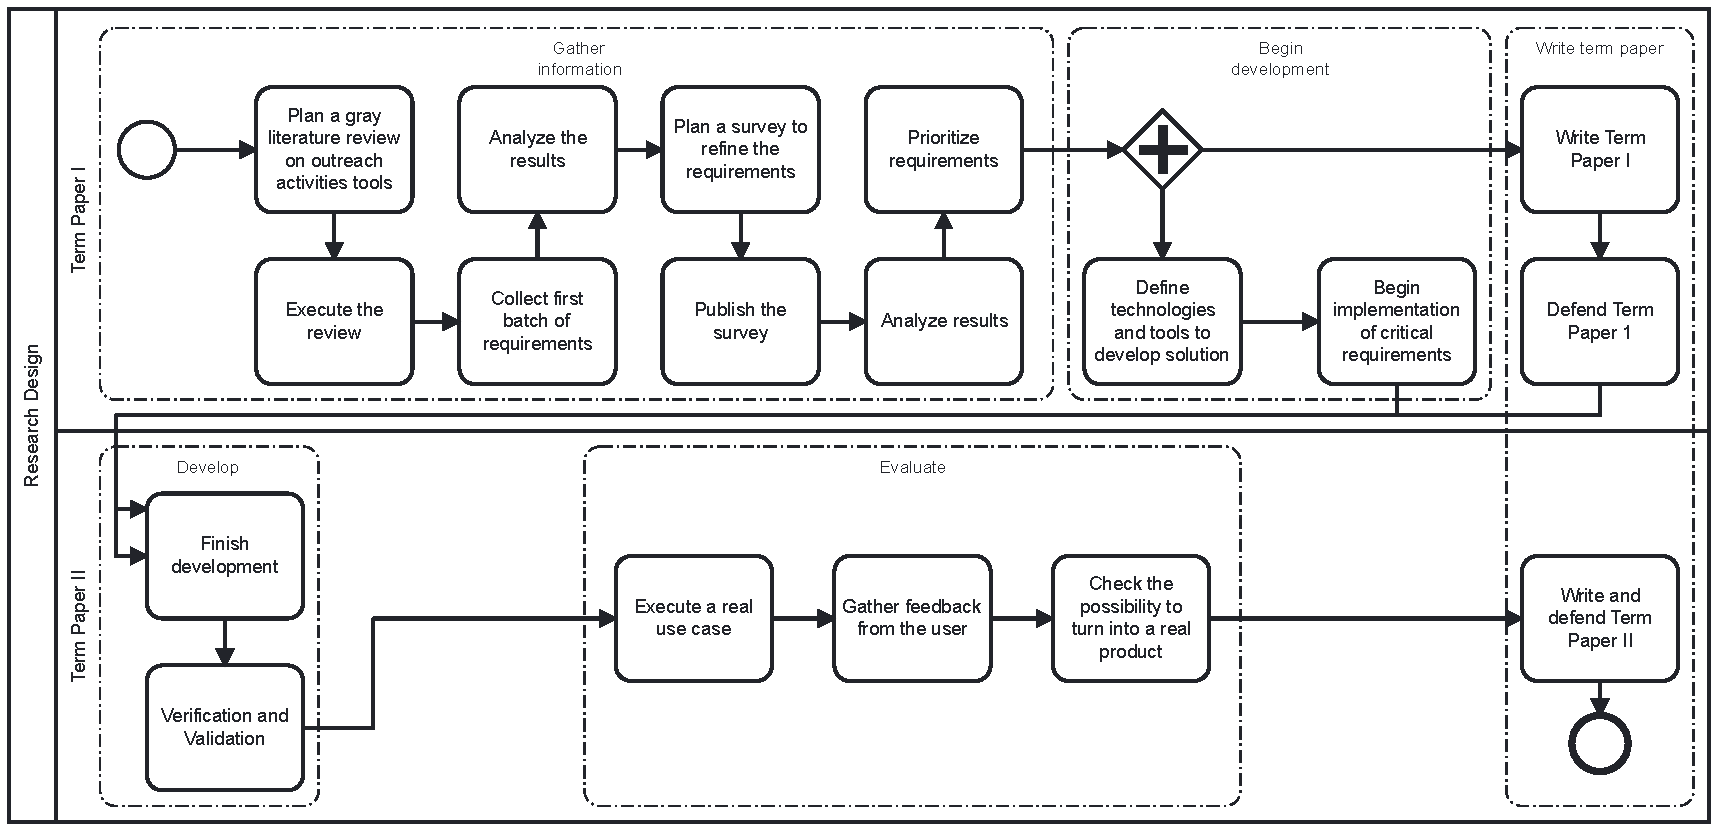
\includegraphics[width=11cm, ]{img/2-research design.pdf}
  \end{figure}
\end{frame}